% Pour le site Cadremploi, cette requête est une requête ElasticSearch et est donc extrêmement rapide.
% La partie de Read de l'application se résume ainsi à la simple exécution d'une requête ES et au remplissage de DTO.
%-------------------------------------------------------------------------
\subsection{Implémentation}
\label{sub:Implémentation}
L'équipe Cadremploi a été en mesure de mettre en place cette architecture particulièrement intéressante dans le projet Espace Recruteur en se basant sur plusieurs concepts tirés du Domain Driven Design (DDD) et en utilisant diverses technologies récentes.
Notamment, l'utilisation des acteurs Akka a permi une gestion confortable et performante des événements que je traiterai dans les parties suivantes et l'utilisation d'ElasticSearch a offert une rapidité en lecture importante.

%-------------------------------------------------------------------------
\subsubsection{La séparation effective de la lecture et de l'écriture}
\label{subs:La séparation effective de la lecture et de l'écriture}
L'espace recruteur utilise deux moyens différents pour accéder à la donnée en lecture et en écriture.
En effet, les données reçues des commandes sont stockées dans une base PostreSQL sous forme d'événements tandis que les données utilisées en lecture sont accessibles via un index ElasticSearch.
Cette utilisation de technologies dédiées est ainsi bien plus performant pour chaque type d'action.
%-------------------------------------------------------------------------
\paragraph{L'écriture}
\label{par:L'écriture}
Les données sont stockées sous forme d'événements dans une base de données PostgreSQL et toute la partie écriture de l'application se fait sur cette base.
Les données ne peuvent y être qu'insérées (append only), c'est à dire que les données déjà présente ne sont jamais modifiées.
Une ligne de cette base représente un événement et contient ainsi la donnée relative à cet événement, sa date d'application sur le système ainsi que l'identifiant de l'aggrégat sur lequel il s'applique.
C'est ainsi sur cette base que repose la structure d'Event Sourcing de notre application.
En effet, l'idée fondamentale de l'Event Sourcing est qu'en enregistrant chaque événements survenant sur un système, on peut retrouver l'état de ce système à tout instant; cette base est la liste de tous les événements ayant eu lieu depuis le démarrage de l'application et est donc centrale à notre application.
% TODO réplication
%-------------------------------------------------------------------------
\subparagraph{Cohérence de la base}
Comme expliqué précédemment, plusieurs contrôles sont effectués avant la validation d'une commande pour assurer la validité de l'information insérée et donc la cohérence de la base.
En effet, cette "liste d'événement" est la base de l'application de l'Espace Recruteur et l'information qui y est présente est utilisée pour construire/reconstruire l'application.
Une corruption de la donnée qui y est présente n'est donc pas envisageable.
Ce type de stockage est néanmoins extrêmement rapide, ce qui nous intéresse du point de vue des commandes puisqu'on essaye de donner à l'utilisateur un retour quasi immédiat sur son action.

%-------------------------------------------------------------------------
\paragraph{La lecture}
\label{par:La lecture}
Les données disponibles en lecture le sont depuis un index ElasticSearch qui est mis en place au démarrage de l'application.
\label{def:ElasticSearch}ElasticSearch est un moteur de recherche open source qui permet de disposer en quelques minutes seulement d'un moteur de recherche clusterisé, automatiquement sauvegardé et répliqué et interrogeable via une API REST.
%-------------------------------------------------------------------------
\subparagraph{Mise à jour asynchrone de la couche}
Cet index est mis à jour de manière asynchrone à la réception d'une intention de l'utilisateur.
En effet, parallèlement à l'ajout d'un événement en base de donnée (Postgre), un message Akka est envoyé sur un bus interne à l'application et sera utilisé pour mettre à jour l'index ElasticSearch.
L'envoi et le traitement de ce message sont fait, par les projections, de façon totalement asynchrone, de manière à ne pas ralentir l'envoi d'un feedback à l'utilisateur.
Nous avons vu précédemment que l'exécution d'une commande est soumise à plusieurs contrôles, mais une fois que ceux-ci sont passés, l'action est validée et il est possible d'envoyer un retour à l'utilisateur de manière synchrone pour que celui-ci sache que son action a bien été prise en compte.
Le traitement interne de l'action ne doit pas ralentir l'envoi de ce feedback.
%-------------------------------------------------------------------------
\subparagraph{Consistence des données}
Il est nécessaire que les données de la couche de lecture soient constamment mises à jour de manière à rester consistantes avec les données présentes dans la base de données PostgreSQL sans avoir pour autant à l'interroger.
La souplesse offerte par Akka et sa gestion asynchrone des acteurs permet une mise à jour non bloquante de l'index ElasticSearch.
Cela permet d'offrir à l'utilisateur un feedback immédiat, mais que la mise à jour de l'index ElasticSearch est différée.
Concrètement, on peut affirmer que l'équipe Cadremploi a choisi d'avoir parfois du retard au niveau de sa couche de lecture.
Par exemple, une modification du titre d'une offre depuis son espace recruteur ne pourra être visible sur le backoffice qu'une ou deux secondes après la modification effective.
En effet, pour garantir un retour rapide à l'utilisateur, donc maximiser la réactivité de mon système, la cohérence des données est remise à plus tard (quelques milli-secondes plus tard).
%-------------------------------------------------------------------------
\paragraph{}
En somme, les parties d'écriture et de lecture sont physiquement séparées dans l'application Espace Recruteur de Cadremploi.
On en retire une réactivité forte du point de vue de l'utilisateur recruteur, mais aussi d'une puissance de requêtage importante apportée par l'index ElasticSearch.

%-------------------------------------------------------------------------
\subsubsection{Reste de l'infrastructure}
\label{subs:Reste de l'infrastructure}
Plusieurs outils sont utilisés de manière à faire fonctionner ce modèle, je vais les lister rapidement avant d'expliquer le fonctionnement concret du mécanisme des commandes et des queries au sein de l'application Cadremploi.
\paragraph{Akka}
\label{par:Akka}
\begin{wrapfigure}{r}{0.25\textwidth}
  \begin{center}
    
\includegraphics[width=0.25\textwidth]{Pictures/akka_logo.png}
  \end{center}
\end{wrapfigure}
Akka est un outil se basant sur le modèle des acteurs de manière à offrir une plate-forme permettant de construire des applications concurrentes et scalables.
Ce modèle d'Acteurs permet une abstraction de haut niveau pour implémenter des services concurrents et parallèles, des modèles événementiels performants et non bloquants.
C'est justement ce dont Cadremploi a besoin, puisque le nombre d'utilisateur et donc d'interactions avec le système tendent à être importants.
L'abstraction qu'offre Akka et son modèle d'acteurs couplé à l'utilisation du langage Scala a permi d'écrire un code élégant et performant.
\paragraph{Kafka}
\label{par:Kafka}
Kafka est un service offrant la fonction de système de message de type publish/subscribe partitionné et répliqué.
Il permet un traitement en temps réel de la donnée mais offre aussi la possibilité de gérer des files d'attentes entre autres.
\begin{wrapfigure}{l}{0.25\textwidth}
  \begin{center}
    
\includegraphics[width=0.15\textwidth]{Pictures/kafka_logo.jpg}
  \end{center}
\end{wrapfigure}
Cet outil est utilisé au sein de Cadremploi puisqu'il offre un bus de données permettant, à la réception d'une commande, de publier un événement (publish), et à chaque projection ayant souscrit à ce type d'événement (subscribe), de le recevoir et d'agir en fonction de son contenu.
Akka gère généralement ça grâce à son implementation d'un EventBus, mais l'application Cadremploi a besoin de discuter avec des applications externes, notamment le Backoffice mentionné précédemment, et c'est Kafka qui fait le lien entre ces différentes applications.



%-------------------------------------------------------------------------
\subsubsection{Les commandes}
\label{subs:Les commandes}
Dans l'espace recruteur de Cadremploi, une commande représente une action venant de l'utilisateur visant à modifier les données le concernant.
Cela peut s'agir de son profil utilisateur, des entreprises qu'il gère ou bien des annonces qu'il a écrites.
%-------------------------------------------------------------------------
\paragraph{L'interface}
\label{par:L'interface}
%%TODO image d'un champ rempli, de la requête Json générée et de l'envoi à l'application
%-------------------------------------------------------------------------
\subparagraph{Envoi d'une commande}
\label{subp:Envoi d'une commande}
L'interface de l'espace recruteur est pensée de sorte à ce que le recruteur qui l'utilise envoit des commandes à l'application de manière transparente.
En effet, à chaque champ du formulaire rempli, une requête Ajax contenant les informations relatives à la modification effectuée est envoyée à l'application.
Concrètement, on utilise un élément d'AngularJS appelé watcher permettant d'enregistrer un callback à exécuter lorsqu'une expression ciblée est modifiée.
Cette technologie permet des appels asynchrones à la fonction de callback et offre donc une fluidité d'utilisation à l'application.
Le but de la fonction de callback est d'effectuer des vérifications côté client de la saisie du recruteur avant de générer un appel REST de type POST à destination du serveur de l'application.
Cet appel sera interprété et traduit en une commande que l'on tentera d'exécuter.
%-------------------------------------------------------------------------
\subparagraph{Réception de la réponse}
\label{subp:Réception de la réponse}
La réponse retournée par le serveur après une requête REST permet d'informer le client de la bonne réception de son action.
Lors de la saisie d'une offre, une bulle d'information est affichée uniquement si la réception s'est mal passée puisqu'on ne souhaite pas bombarder le client d'information.
\begin{figure}[h]
  \begin{center}
    
\includegraphics[width=0.4\textwidth]{Pictures/implementation/capsule_orange.png}
    \caption{Message d'erreur}
    \vspace{1em}
    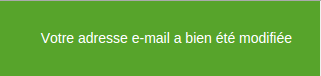
\includegraphics[width=0.4\textwidth]{Pictures/implementation/capsule_verte.png}
    \caption{Message de succes}
  \end{center}
\end{figure}
L'information sur le retour est affichée dans tous les cas quand la modification concerne le profil de l'utilisateur.
Ce retour est très rapide puisque le gros du traitement côté serveur, est fait de manière asynchrone.
%-------------------------------------------------------------------------
\paragraph{Backend}
\label{par:Backend}
L'utilisation du pattern Command est rendu possible grâce à plusieurs objets.
%-------------------------------------------------------------------------
\subparagraph{Les objets Command}
\label{subp:Les objets Command}
Comme expliqué précédemment, l'équipe Cadremploi a représenté une commande est un appel de méthode encapsulé dans un objet.
Nous avons choisi de décorréler l'exécution de l'action et la description de l'intention de l'utilisateur.
Concrètement, cela signifie qu'une classe se charge de la définition de la commande, tandis qu'une seconde traitera l'exécution de l'action.
%%TODO schéma UML de la séparation Command/CommandHandler
Ce découpage en Command et CommandHandler est légèrement plus verbeux, mais permet néanmoins de réduire la taille des classes que nous écrivons et offre la possibilité d'un traitement asynchrone.
En effet, on peut imaginer placer les commandes sur une queue qui sera traitée par les CommandHandlers dès que la ressource nécessaire à leur exécution se trouve disponible.
Une logique similaire qui n'est pas encore exploitée par Cadremploi serait d'envisager un mode déconnecté puisqu'il est possible d'exécuter des commandes en local qui seront envoyés sur le serveur et donc traitées effectivement dès que la connexion est récupérée.
%-------------------------------------------------------------------------
\subparagraph{Le command executor}
\label{subp:Le command executor}
Un exécuteur de commande (ou "CommandExecutor") est une entitée créée pour être utilisée à l'exécution de chaque commande.
Cette classe expose une méthode permettant d'exécuter une commande donnée.
Cet exécuteur se charge de:
\begin{itemize}
  \item retrouver l'aggrégat visé par la commande s'il existe
  \item vérifier que l'auteur de l'action est autorisé à l'effectuer
  \item récupérer le CommandHandler associé à la commande et appliquer son effet
  \item enregistrer les événements générés en base et les diffuser sur les différents bus de donnée.
\end{itemize}
Si une erreur survient lors de l'exécution d'une commande par le CommandExecutor, elle est utilisée pour informer le front directement via des fonctions de récupérations offertes par le framework Play.

%-------------------------------------------------------------------------
\subsection{Les Queries}
\label{sub:Les Queries}
%-------------------------------------------------------------------------
Une query est un objet permettant à l'utilisateur de requêter de la donnée provenant du serveur.
Chaque information provenant de son profil ou de ses annonces provient d'une query.
%-------------------------------------------------------------------------
\paragraph{Backend}
\label{par:Backend}
%-------------------------------------------------------------------------
\subparagraph{Les objets query}
\label{subp:Les objets query}
De même que les commandes, les queries sont aussi des actions encapsulées dans des objets dans l'Espace Recruteur.
Elles sont pour leur part découpées en 3 objets différents:
\begin{itemize}
  \item Query qui est la définition de la requête, il s'agit généralement d'un objet vide, uniquement caractérisé par son nom qui est, tout comme la commande, très explicite.
  \item QueryResult, qui est un conteneur pour le résultat de la requête.
  Il s'agit donc d'une classe contenant un ou plusieurs objets.
  \item QueryHandler, qui tout comme les CommandHandler, sont des objets qui contiennent la méthode d'application de la requête.
  Il s'agit d'une méthode requêtant un index ElasticSearch directement et encapsulant son résultat dans un objet QueryResult.
  Nous avons en effet vu que les données contenus dans les indexes sont utilisable directement et qu'aucun contrôle n'est fait.
\end{itemize}
Le résultat des queries est sérialisé puis directement envoyé au front.
%-------------------------------------------------------------------------
\subparagraph{Le query executor}
De même que le CommandExecutor, le QueryExecutor est une entité exposant une méthode permettant d'exécuter une requête donnée.
Puisqu'aucune modification n'est faite par une "query", la QueryExecutor se charge uniquement de récupérer le handler associé à la requête puis de renvoyer le QueryResult associé.

\paragraph{}
Les exécuteurs de requêtes et de commandes sont utilisées comme des courroies par lesquelles passent toutes les actions de lecture et d'écriture faite sur le système.
Il est ainsi très simple de contrôler à haut niveaux toutes ces transactions.

\subsection{Bilan}
\paragraph{}
Le modèle CQRS permet d'orienter l'architecture vers un système capable de gérer la partie écriture de l'application en ACID (de l'anglais Atomicity, Consistency, Isolation, Durability) et la partie lecture en BASE (de l'anglais Basically Available Soft-State with Eventual consistency).
Cet effort permet d'offrir plus de confort à l'utilisateur, mais aussi plus de flexibilité et de performance à l'application via l'utilisation d'outils dédiés.
\paragraph{}
L'introduction d'événements, via le pattern Event Sourcing, offre de nombreux bénéfices à ce type d'architecture puisqu'il permet de décrire le comportement de l'application avec encore plus de clarté en mettant en avant le dynamisme du modèle.
De plus, cela permet une isolation des responsabilités encore meilleure: ils permettent notamment d'isoler les différents cas de lectures (via les projections).
L'utilisation d'outil récents comme Akka et Kafka permettent une communication intra et inter applications simplifiée, même dans des cas complexes, tout en assurant une scalabilité importante et une clarté du code.

%-------------------------------------------------------------------------
\subsection{Critiques du modèle}
%-------------------------------------------------------------------------
Lors de l'implémentation d'une telle architecture, l'équipe Cadremploi s'est heurté à des problèmes que le modèle théorique ne laissait pas réellement présager.
En effet, le modèle implémenté par notre équipe est plutôt récent et peu d'autres entreprises s'y sont risqués.
La documentation et les retours d'expérience à ce sujet sont ainsi limités.
Je vais tenter de présenter les difficultés entraînées par ce modèle d'architecture, au delà de son apparence inhabituelle et du changement de mode de réflexion qu'elle demande.
\subsubsection{L'exemple de la migration des événements}
%-------------------------------------------------------------------------
\paragraph{}
Une application reste rarament figée au cours du temps, et le jeune Espace Recruteur de Cadremploi n'échappe pas à cette règle.
Ainsi, les événements écrits à la naissance de l'application sont voués à changer au cours du temps et des modifications y seront apportées.
Il est quasiment certain que les événements existant aujourd'hui seront modifiés, enrichis voire même supprimés pour certain, et qu'ils ne peuvent donc rester totalement statique en base.
La migration des événements contenus dans la base est nécessaire de manière à ne pas figer le comportement de l'application ni devoir être gêné continuellement par des comportements obsolètes dans le futur.
J'ai ainsi travaillé, avec le reste de l'équipe, sur un outil de migration des événements de notre base dans le cas d'une modification de la sorte.

%-------------------------------------------------------------------------
\paragraph{}
L'équipe Cadremploi a écrit ses événements sous forme de classes Scala, expressives, utilisées ainsi lors de la réception de la commande, de la réception par les projections, de l'écriture en base...
Il s'agit d'objets à usage multiple, et leur modification entraîne des changements importants.
En effet il est nécessaire de modifier les événements déjà présents en base de manière à ce qu'ils soient désérialisables même dans leur nouvelle version.
Pourtant, cette pratique est contraire à la non-modification des données de cette base.
%-------------------------------------------------------------------------
\paragraph{}
Une solution consistante avec le modèle serait de rajouter des événements "de migration" à la suite de ceux existant permettant de modifier les projections.
Mais si une projection, suite à un problème technique, se doit d'être rejouée, il sera nécessaire de lire les données depuis la base des événements pour la reconstruire.
À ce moment là, la désérialisation des événements pour que l'application puisse les interpréter sera nécessaire; leur version ayant changé, cette désérialisation ne sera plus possible.
Il est alors impossible de rejouer correctement une projection via cette méthode.
L'équipe Cadremploi se voit donc contrainte de mettre à jour les événements de cette base, modifiant leur structure sérialisée.
%-------------------------------------------------------------------------
\paragraph{}
La solution à ce problème serait de ne plus utiliser de classe et d'utiliser uniquement du Json (ce en quoi sont aujourd'hui sérialisé les événements en base).
Cela entraînerait certainement des complications à chiffrer puisque le code perdrait en élégance, l'utilisation des traits, pattern matching et autres bénéfices offerts par le langage Scala n'étant plus accessibles.
%-------------------------------------------------------------------------
\subsubsection{Bilan}
%-------------------------------------------------------------------------
\paragraph{}
Le modèle CQRS couplé à de l'Event Sourcing offre de très nombreux bénéfices.
Il offre notamment beaucoup de clarté de code mais multiplie pour ce faire les lignes nécessaire à l'implémentation de la solution.
Manquant de documentation sur le sujet, certains éléments de simplification peuvent paraître intéressants à première vue, mais avoir une conséquence inattendue et gênante.
En plus de ce cas de migration des événements demandant la modification de la base et donc de l'historique, qui devrait demeurrer immutable, de l'application, des dérives du modèle telles que la création de commandes avec une valeur de retour par exemple, sont survenues au cours du développement de l'Espace Recruteur.
%-------------------------------------------------------------------------
\paragraph{}
Ce type d'architecture étant récente, l'implémentation du modèle CQRS + Event Sourcing a demandé à notre équipe la création d'une sorte de framework maison.
Cette création, quasi expérimentale et parallèle au développement de l'application Espace Recruteur, s'est retrouvé rapidement bloquante pour la validation de nouvelles tâches.
En effet, des éléments innatendus, car peu ou pas mentionné dans les documents sur lesquels se base notre équipe pour mettre en place ce framework, ont demandé parfois plusieurs semaines de développement.
%-------------------------------------------------------------------------
\paragraph{}
Néanmoins, lorsque les différents outils permettant de migrer les événements ou rejouer les projections seront mis en place, notre équipe pourra enfin profiter des nombreux avantages offerts par ce modèle.
